% !Mode:: "TeX:UTF-8"
\chapter{可见光多波段通信系统概述}
\section{引言}
得益于LED灯在照明市场的风行,使得兼顾通信和照明两重功能的可见光通信技术受到了越来越多的关注。基于LED的可见光通信因其绿色环保、高速便捷、频谱资源不受限制等优点,极有可能在未来的无线通信中占有一席之地,特别是诸如机舱、医院和矿井这些特殊应用场景下。本章将先介绍可见光通信的基本原理,包括基础硬件发光二极管(LED)和光电二极管(PD)的基本工作原理及可见光通信系统模型,然后将概述OFDM在可见光通信中的应用,并且比较ACO-OFDM及DCO-OFDM之间的区别,最后将简介自适应传输技术及其在可见光通信中的应用。
\section{室内可见光通信基本原理}
\subsection{可见光系统模型}
与传统的无线通信技术通过调幅、调频或调相技术将信息调制到射频载波上不同,可见光通信利用的是人眼可见的波长在380 nm 到780 nm之间的电磁波来传输信息,并且是使用强度调制(Intensity Modulation,IM)、直接检测(Direct Detection,DD)技术。如\autoref{fig:BasicOpticalSystem}所示,在发射端,利用LED灯的易于调制性,在线性范围内,LED 的发光强度与输入电流功率成正比,将电信号调制到LED发光强度上;在接收端,利用PD的输入反向电流功率与接收到的光强成正比的特性,用光电二极管去检测LED发光强度的变化,将光信号转换成电信号。
\begin{figure}[htbp]
    \centering
    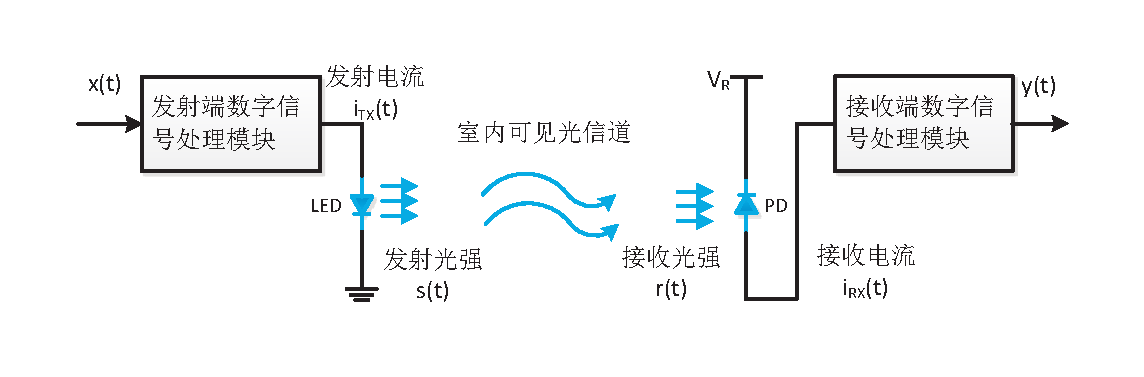
\includegraphics[width=\textwidth]{figures/chapter-2/BasicOpticalSystem.eps}
    \caption{光无线通信系统模型}
    \label{fig:BasicOpticalSystem}
\end{figure}
如\autoref{fig:BasicOpticalSystem}所示,在电信号域(Electrisity domain)发射端输出电压信号$x(t)$经过发光二极管后变成LED的电流$i_{TX}(t)$信号,接收端光敏二极管PD输出电流$i_{RX}(t)$,其最后转换成接收信号$y(t)$ ,在光信号域(Light Domain),首先在发射端发光二极管LED的电流信号$i_{TX}(t)$ 转变为发光强度$s(t)$,经过光信道后,在接收端光电二极管PD收到的光强信号为$r(t)$,经过光电转换,得到电流$i_{RX}(t)$。
所以在实际可见光通信系统中,信号传输由电光变换,光通道传输及光电变换三个过程组成,如\autoref{fig:BasebandModle}所示,接收端信号$y(t)$ 可以表示为:
\begin{equation}
    y(t)=x(t)\otimes h_1(t)\otimes h_2(t)\otimes h_3(t)+z(t)
\end{equation}
其中,$x(t)$表示发射端基带电压信号,$h_1(t)$表示电光转换系统的时域信道冲激响应(Channel Impose Response,CIR),$h_2(t)$表示可见光信道的时域信道冲激响应,$h_3(t)$表示光电转换系统的时域信道冲激响应
\cite{Yangxuecheng2015},
$z(t)$表示信道加性白高斯噪声(Additive White Gaussian Noise,AWGN),符从$z(t)\sim N(0,N_0/2)$分布,$N_0$为其功率谱密度,$\otimes$表示卷积运算。可见光通信系统的噪声,通常主要由热噪声和散弹噪声
\cite{Chenchunyan2014}。热噪声是一种高斯白噪声,在传统的射频无线通信系统中是很常见的。
散弹噪声也可以建模为白高斯噪声来处理,因为两个独立分布的高斯噪声还是高斯的,故我们可以将系统噪声统一建模为与信号独立的高斯白噪声。

\begin{figure}[htbp]
\centering
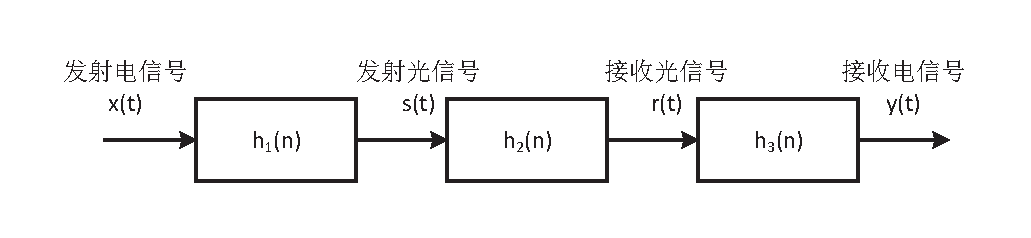
\includegraphics[width=0.9\textwidth]{figures/chapter-2/BasebandModle.eps}
\caption{光无线通信系统基带处理模型}
\label{fig:BasebandModle}
\end{figure}

\subsection{光电元器件简介}
如前文所述,可见光通信与传统的无线通信最大的区别在于调制与信号检测上,射频无线通信必须把基带信号通过调幅、调频或者调相技术调制到高频率的载波上,在接收端再下变频得到基带信号。但目前可见光通信器件技术还不能直接去调制光的幅度、频率或者相位,而是使用发射端强度调制和接收端直接检测技术。在发射端,需要电光转换器件将电信号转换成光信号,在室内可见光通信中用到的主要是发光二极管LED,LED就是调制器,其工作线性范围是一个非常重要的指标,因为如果输入信号的动态变化范围较大,超出LED的线性调制范围,则会发生非线性失真,将严重影响通信性能,在可见光OFDM系统中尤其要注意这点,另外,LED的响应时间是另一个重要指标,响应时间断的LED 能够被更高频率的信号调制,也就意味着带宽增加、通信速率增高。在接收端,需要光电转换器件将光信号再变成电信号以进行解调解码,目前大量使用的是光电二极管PD,光电二极管的PN结面积相对比较大,以便接收更多的入射光,其在反向电压的作用下,没有光照时,反向电流非常小,称为暗电流;在有光照时,反向电流急速增大,并且在一定范围内反向电流功率与光照强度成正比。本节将详细介绍发光二极管和光电二极管的通信特性。
\subsubsection{电光转换器件}
目前在光通信领域使用得电光转换器件主要有激光二极管(Laser Diode,LD)和发光二极管LED两类,这两种器件的性质差异很大,应用场景也不同。激光二极管响应速度非常快,但是线性区间非常小,几乎只有关闭和激发两种状态,而且发光角度较小,通信时需要发射端与接收端对准,所以一般用于高速光纤通信中。这里我主要讨论室内无线光通信使用的发光二极管LED。

发光二极管LED是一种掺杂了镓(Ga)、砷(As)和磷(P)等化合物的半导体器件,它跟普通的二极管一样,具有单向导电性,内部有PN节,P区含有多余的电子,N区则有多余得空穴。当给发光二极管加正向电压时,P区的高能电子与N区的空穴结合发生能级跃迁变为低能电子,根据能量守能,其将向外辐射电磁波,并且包含波长在380 nm到780 nm 之间的人眼可见的电磁波,具体辐射电磁波的波长主要由掺杂物的种类相关,这就是LED发光的基本原理。

\begin{figure}[htbp]
    \centering
    \subfloat[磷激发型LED光谱图]{
        \label{fig:OSTAR-Spectrum}
        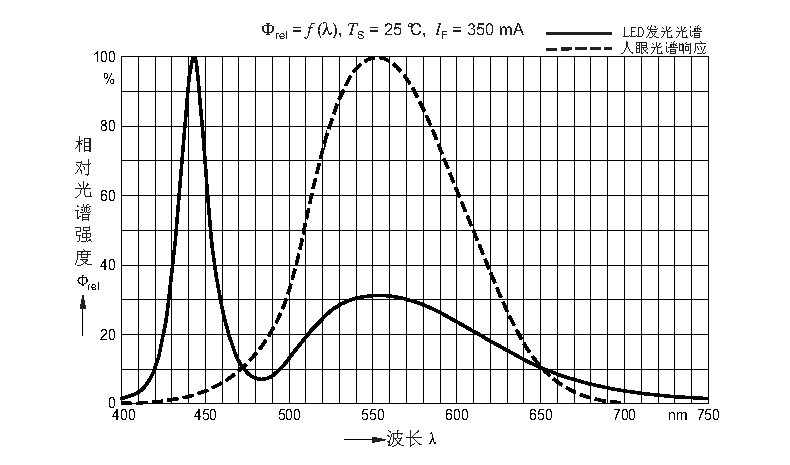
\includegraphics[width=0.5\textwidth]{figures/chapter-2/LEUWS2LN-RelativeSpectralEmission.eps}
    }
    \subfloat[RGB三原色混光型LED光谱图]{
        \label{fig:RGB-Spectrum}
        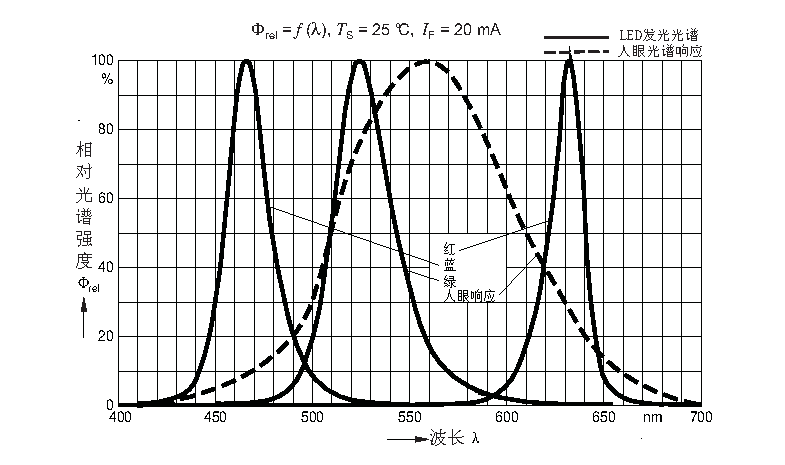
\includegraphics[width=0.5\textwidth]{figures/chapter-2/LRTBR98G-RGB-RelativeSpectralEmission.eps}
    }
    \caption{两种白色LED光谱对比图}
    \label{fig:WhiteLED}
\end{figure}

众所周知,白光是一种混合光,故我们日常用于照明的白光LED灯发出的白光也是由几种光合成的。现在市面上的白光LED主要有两种类型。一种是磷光激发型,由蓝光LED激发荧光物质发出黄光,然后蓝光与黄光混合成我们人眼看到的白光;另一种是多色混合型,由多个LED发出不同颜色的光直接合成为白光,这种类型常见的红绿蓝(RGB)LED灯内部就含有三块晶片,分别发红光、绿光和蓝光。图\ref{fig:OSTAR-Spectrum}所示是德国OSRAM公司生产的磷光激发型发光二极管Lighting Plus LE UM S2LN的相对光谱分布图\cite{LE2011},图中峰值位于445 nm处的是蓝光LED发出的蓝色光波,而峰值位于555 nm处的是蓝光激发荧光物质产生的黄光。因为激发荧光物质发黄光的响应时间过长,在使用磷光型LED 进行可见光通信时,一般同时会在接收端加蓝色滤光片,滤掉响应过慢的黄光,所以虽然我们人眼看到的是白光,但是信号其实只调制在蓝光上,这就是前文中提到单色白光LED通信。图\ref{fig:RGB-Spectrum}所示多色混合型LED的相对光谱分布图\citep{LRTB2011},其具体型号为LRTB R98G,同为OSRAM生产。图中可见红绿蓝三种色光的峰值分别位于635 nm、525 nm和465 nm 处,与林光激发型LED不同的是,红绿蓝三种色光分别由三种不同的LED晶片产生,都有很好的响应速度,我们可以对这三种色光分别调制,达到同时传输三路数据的目的,这样可以大大加大传输速率,即为前文所述的多色白光无线通信系统,也是本课题主要研究对象。


因为基于多色混合型LED的可见光通信系统能将各基色独立调制,总速率为各基色速率之和,所以相对于使用磷光激发型LED的单色光通信系统速率优势明显。现在也有专门的公司设计适合可见光通信的LED,如硅谷光擎(LED Engin),其生产了多种通信特性优异的多色混合型LED,如\autoref{fig:LED_LZ4_SputrcalPower} 所示为型号为LZC-03MA07的多色混合型LED的相对光谱功率分布和绝对光谱功率分布。从图\ref{fig:LED_LZ4_relativeSputrcalPower}中可以看出该白光LED 其由四种基色组成,分别为红(Red)、绿(Green)、蓝(Blue)和黄(Yellow),其中黄色有时也称为琥珀色(Amber),并且各基色光之间隔离明显,相互之间的干扰很少,同时图\ref{fig:LED_LZ4_absoluteSputrcalPower}说明各基色的发光功率相差明显,在设计多色光通信系统时也可以优化各个基色光发射功率,减少干扰,这个是我们后面研究的内容。
\begin{figure}[h]
    \centering
    \subfloat[LZC-03MA07相对光谱功率分布]{
        \label{fig:LED_LZ4_relativeSputrcalPower}
        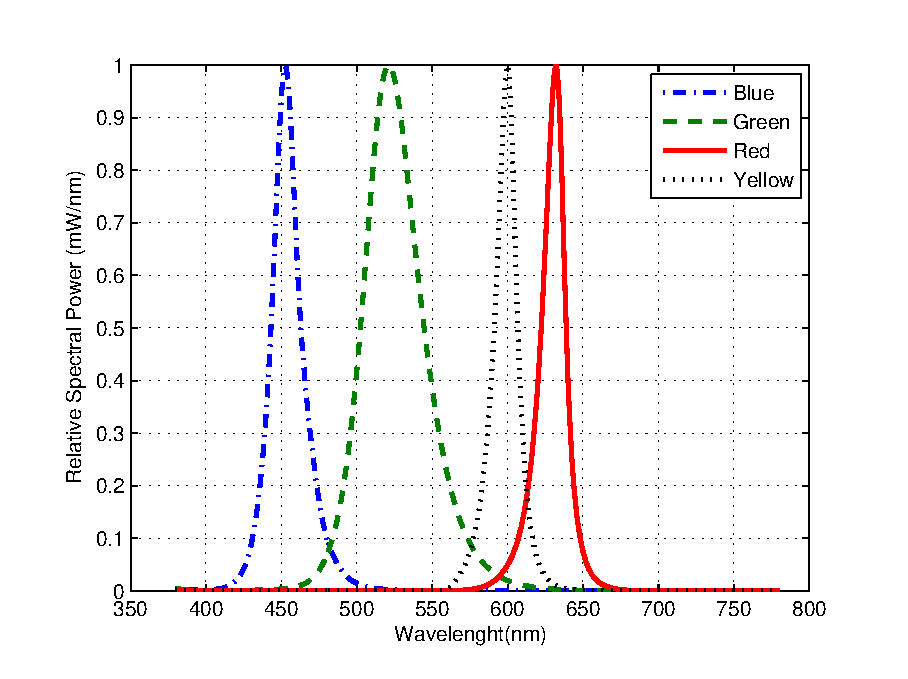
\includegraphics[width=0.5\textwidth]{figures/chapter-2/LED_LZ4_relativeSputrcalPower.eps}
    }
    \subfloat[LZC-03MA07绝对光谱功率分布]{
        \label{fig:LED_LZ4_absoluteSputrcalPower}
        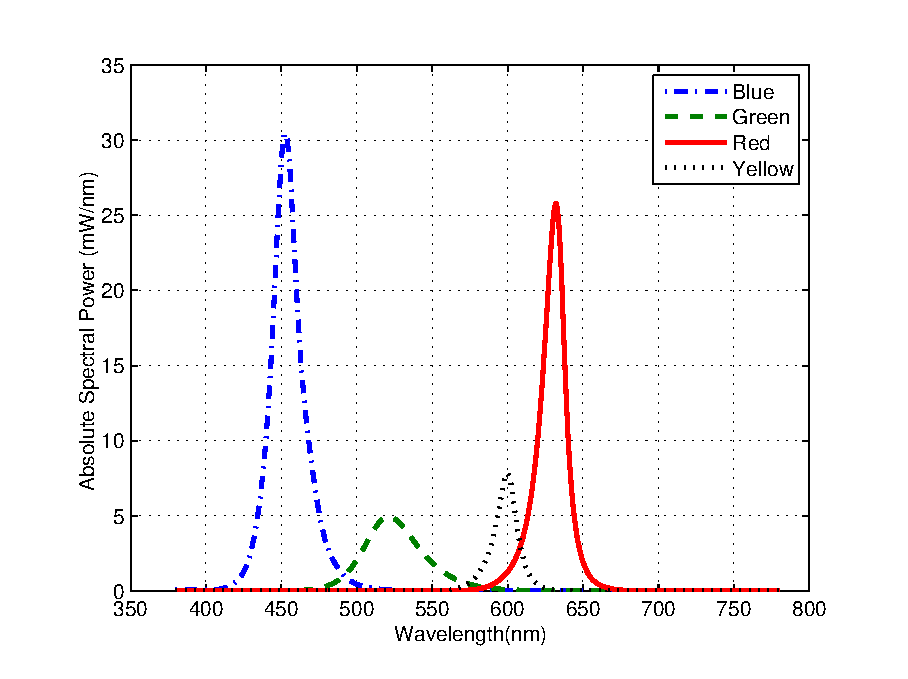
\includegraphics[width=0.5\textwidth]{figures/chapter-2/LED_LZ4_absoluteSputrcalPower.eps}
    }
    \caption{LZC-03MA07光谱功率分布}
    \label{fig:LED_LZ4_SputrcalPower}
\end{figure}

对于电光转换器件LED而言,我们除了要注意体面提到的线性范围和响应时间这两个指标之外,还要考虑LED的特性随温度的变化,如\autoref{fig:LZC_temprature}所示\cite{LZC2013},图\ref{fig:LZC_relativeLightOuput}表明随着温度的升高,LED的输出光功率降低,但是各基色光功率降低的幅度不相同,其中黄光(Amber)下降得最快,单温度升高到120 $^{\circ}$C时,输出功率降到常温下的20\%;而蓝光(Blue)受到的影响较小,功率输出变化不明显。受温度影响的还有各基色的主波长,主波长是指各基色光谱功率分布的峰值位置,如蓝光对应的是450 nm。如图\ref{fig:LZC_wavelengthShift}所示,也是黄光主波长变化最快,波长的漂移将导致接收端的滤光片效果降低,从而限制了总体的接收信噪比(Signal Noise Ratio, SNR)。故在设计可见光通信系统硬件时也要特别留意给LED散热,现在普遍的做法是将LED 安装在散热面积很大的金属灯头上。
\begin{figure}[h]
    \centering
    \subfloat[LZC-03MA07各基色相对输出光功率与温度的关系]{
        \label{fig:LZC_relativeLightOuput}
        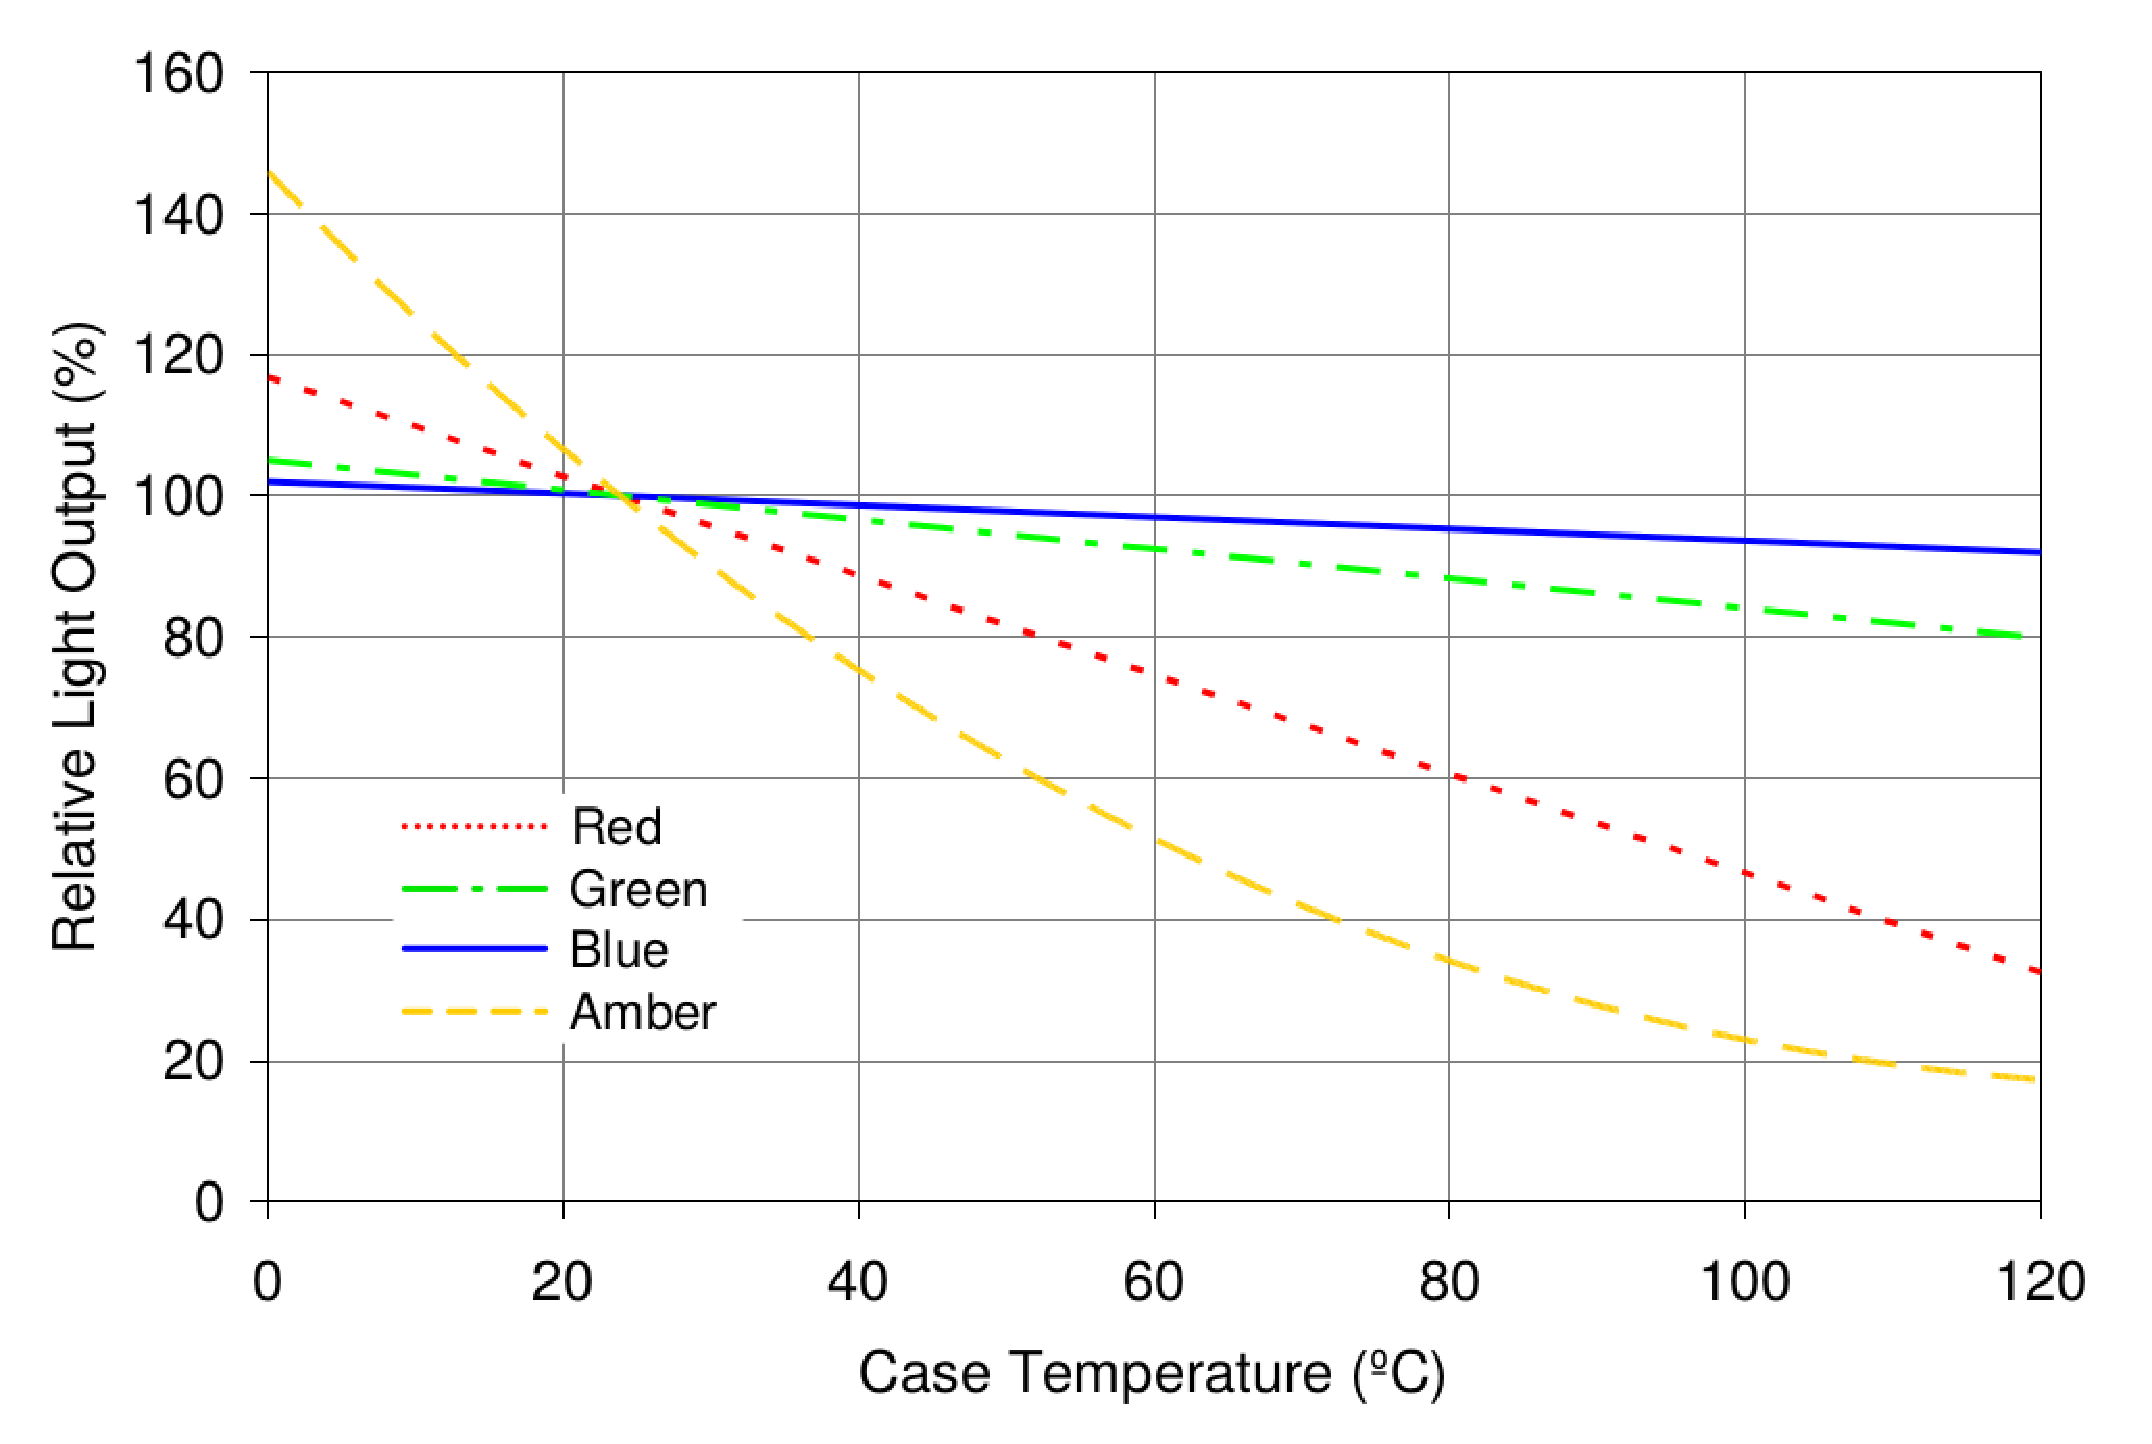
\includegraphics[width=0.5\textwidth]{figures/chapter-2/LED_Temperature_Light_Output.eps}
    }
    \subfloat[LZC-03MA07各基色主波长偏移量与温度的关系]{
        \label{fig:LZC_wavelengthShift}
        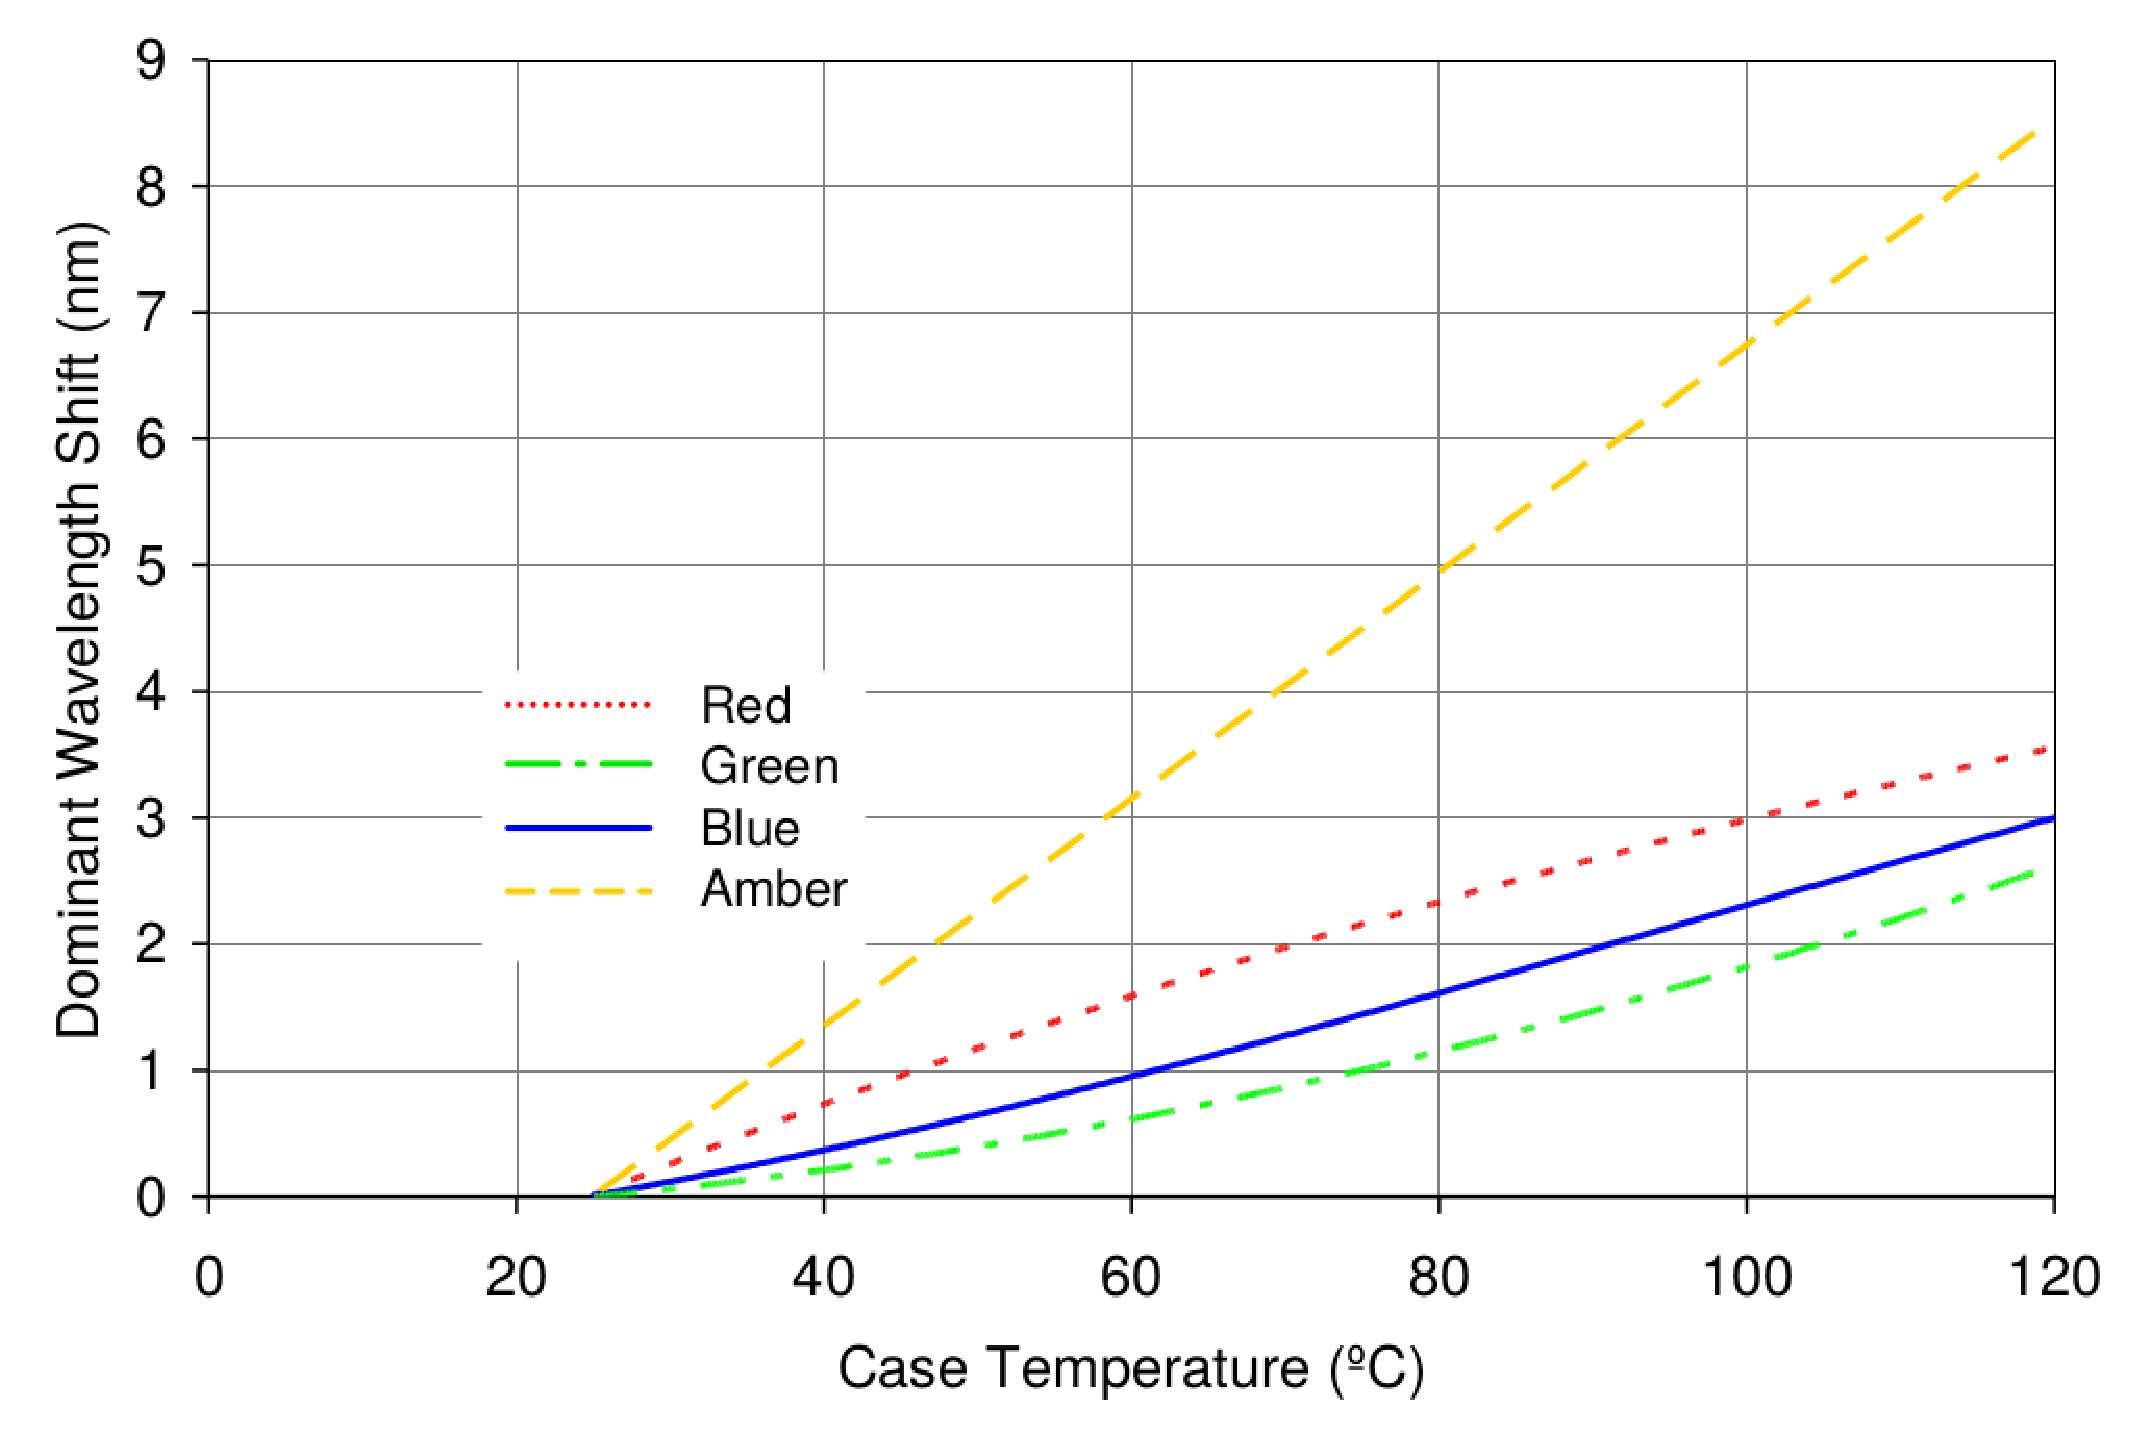
\includegraphics[width=0.5\textwidth]{figures/chapter-2/LED_Temperature_Wavelength_Shift.eps}
    }
    \caption{LZC-03MA07特性随温度变化关系}
    \label{fig:LZC_temprature}
\end{figure}

\subsection{光电转换器件}
现在使用最多的光电转换器件是光电二极管(PD)。光电二极管跟普通的二极管一样,也是一种含有PN节的半导体器件,只是会把PN节中的耗尽区通过某些方式暴露出来以接受光照。所谓耗尽区是在生产二极管时,在P区和N区交界的位置,N区的电子会移向P 区并与空穴结合,这个P区与N区交界的区域就称为耗尽区。但是耗尽区不会持续增加,因为N区的一个自由电子离开它的母体原子,原子就变成了正离子;同理,当自由电子进入P区并与其中的原子结合时,该原子就成为了负离子,离子形成电势阻止更多电子穿过耗尽区。在光电二极管中,耗尽区受到光照,由于光电效应,电子被激发,形成电子-空穴对,在方向配置电压的作用下形成反向电流,这就是光电二极管基本工作原理。
\begin{table}[htbp]
    \caption{PIN 与 APD光电二极管对比}
    \label{tab:PIN_APD_Comparsion}
    \centering
    \begin{tabular}{lllll}
        \toprule
         & PIN & APD \\
        \midrule
        光电增益       & 一般   &雪崩效应    \\
        调制带宽       & 最高几百MHZ  &最高几十GHZ    \\
        线性动态范围   & 较宽  &较窄    \\
        温度敏感度    & 不敏感  &敏感    \\
        制作工艺    &简单 &复杂    \\
        价格    & 低  &高    \\
        \bottomrule
    \end{tabular}
\end{table}

目前在可见光通信中应用的光电二极管有PIN型和雪崩型(Avalanche photodiode,APD)两种,PIN型光电二极管就是在普通的光电二极管的P区和N区之间加入了低掺杂度的I 区,使得耗尽区变厚了,从而缩短了其响应时间,并且提高了截止频率,其调制带宽可达数百兆赫兹,能够适应高速通信系统的要求。同时PIN 型二极管还有线性范围宽、制作工艺简单及价格低等优点。雪崩型光电二极管比较特殊,它的工作原理是在其P区和N区两端加了反向高电压,当有光照射耗尽区产出自由电子和空穴时,在反向高压的作用下,电子和空穴高速碰撞晶格原子,产生更多的电子和空穴,此过程像“雪崩”一样继续下去,从而产生了很大的反向电流。雪崩型光电二极管的优点是灵敏度高、增益高及带宽高,但是制造工艺复杂,价格较贵。PIN型和雪崩型光电二极管的比较如下表\ref{tab:PIN_APD_Comparsion}所示。


\subsection{滤光片}
如前所述,在使用磷光激发型LED的单色光通信系统中,我们要滤掉响应时间过长的黄光只取携带信息蓝光;在使用多色混合型LED 的多色光通信系统中,我们要在每个基色上调制信息,在接收端要把每个基色分别提取出来进行数字信号处理。这些过程要需要一个光学元件——滤光片,准确来说应该是带通滤光片。带通滤光片只允许较窄波长范围的光通过,常见的是法布里-珀罗型滤光片,它实质 上是一个法布里-珀罗标准具(见法布里-珀罗干涉仪)。具体结构为:玻璃衬底上涂一层半透明金属层,接着涂一层氟化镁隔层,再涂一层半透明金属层,两金属 层构成了法布里- 珀罗标准具的两块平行板。当两极的间隔与波长同数量级时,透射光中不同波长的干涉高峰分得很开,利用别的吸收型滤光片可把不允许透过的光 滤掉,从而得到窄通带的带通滤光片,其通频带宽度远比普通吸收型滤光片要窄\cite{OpticalFilter}。
\begin{figure}[htbp]
    \centering
    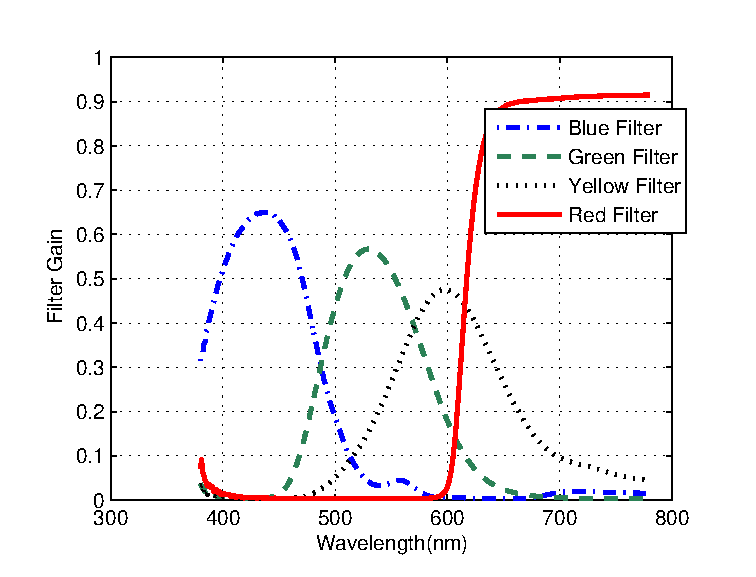
\includegraphics[width=0.8\textwidth]{figures/Chapter-2/MulticolorFilterGain.eps}
    \caption{滤色片滤色性能}
    \label{fig:MulticolorFilterGain}
\end{figure}
类型于滤波器对于射频无线通信的作用,滤光片也对可见光通信系统的性能有着重要的影响,但是精密的滤光片虽然性能优良,但制造工艺复杂、价格昂贵,不利用可见光通信技术的推广,所以在可见光通信中一般会选择价格一般但性能稍差的滤波片,然后借助数字信号处理技术来弥补滤光片性能的不足。本课题搭建的硬件平台发射端使用的是前面提到的混合型LED——LZC-03MA07,接收端使用四块滤光片滤出四个基色,分别是蓝光滤光片DTB435、绿光滤光片DTB530、黄光滤光片DTB600和红光滤光片HB610,它们的滤光带通增益如
\autoref{fig:MulticolorFilterGain}所示,其中除红光滤光片是低通滤光片外(对频率而言),其他三个都是带通的,各滤光片对光信号都有一些衰减,其中黄光滤光片的衰减最大,并且各色之间都有一些串扰。
\autoref{fig:MultiColorReceiveredFilter}所示是接收端未加滤光片接收信号和由四个经滤光片提取的四个基色组合的光功率的比较,可以更清楚地看出滤光片的功能和对信号的衰减。
\begin{figure}[htbp]
    \centering
    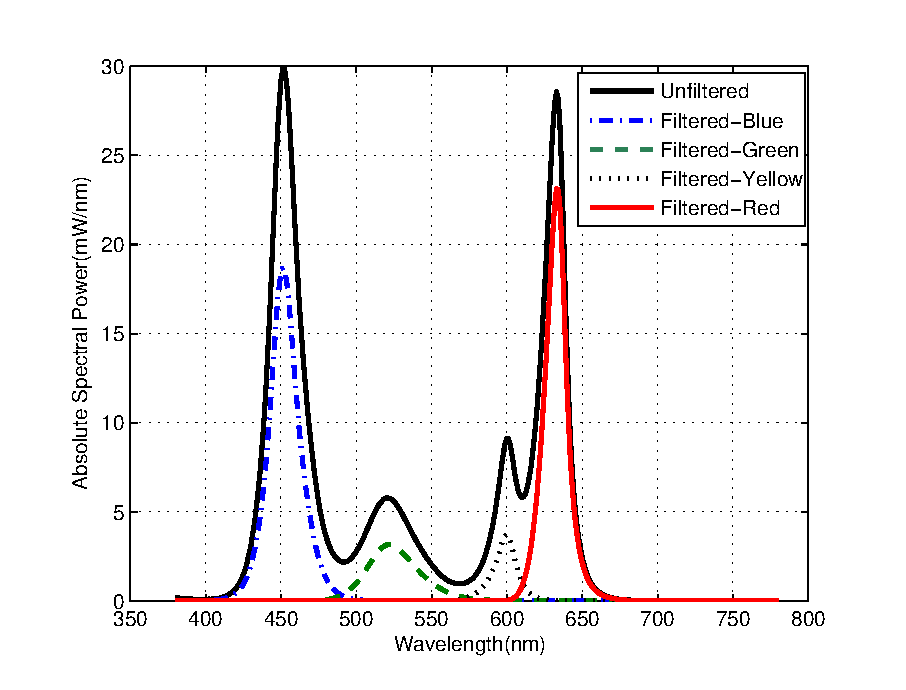
\includegraphics[width=0.8\textwidth]{figures/Chapter-2/MultiColorReceiveredFilter.eps}
    \caption{接收端滤色后光功率谱}
    \label{fig:MultiColorReceiveredFilter}
\end{figure}
\section{OFDM技术在室内可见光通信中的应用}
\subsection{OFDM技术简介}
正交频分复用(OFDM)是一种多载波调制技术,是一种能有效地对抗频率选择性衰落途径,而且频谱利用率较高,实现简单,在很多现代通信系统中得到了广泛的应用,如DSL、WIFI及LTE等。OFDM技术发展历程及其应用如
\autoref{fig:HistoryOfOFDM}所示,最早由美国贝尔实验室的Chang 在1966 申请的专利“正交频分复用数字传输系统”提出;1969年,Salz和Weinstein研究了使用傅里叶变换来实现OFDM的通信系统;用来抵抗码间干扰的循环前缀(Cyclic Prefix, CP)于1980年加入OFDM系统。这是OFDM技术理论发展最重要的三个节点
\cite{armstrong2009ofdm}。在上世纪80年代中期,人们开始研究OFDM技术在实际通信系统中的应用,1985年,同样来自贝尔实验室的Cimini研究了OFDM用于移动通信的可能性;1987年, Lassalle 和 Alard将OFDM技术推广到无线广播系统,并且揭示了前向纠错编码和OFDM技术结合的重要性,对于广播通信工程师而言,OFDM技术也称为C-OFDM(Coded OFDM);最先提出在有线通信中使用OFDM技术的是来自斯坦福大学的Cioffi等人,同时他们展示了OFDM可以作为数字用户线路(Digital Subscriber Line, DSL)的一种替代调制方式;如绪论所述,OFDM近年来也开始被应用于光通信中。
\begin{figure}[htbp]
    \centering
    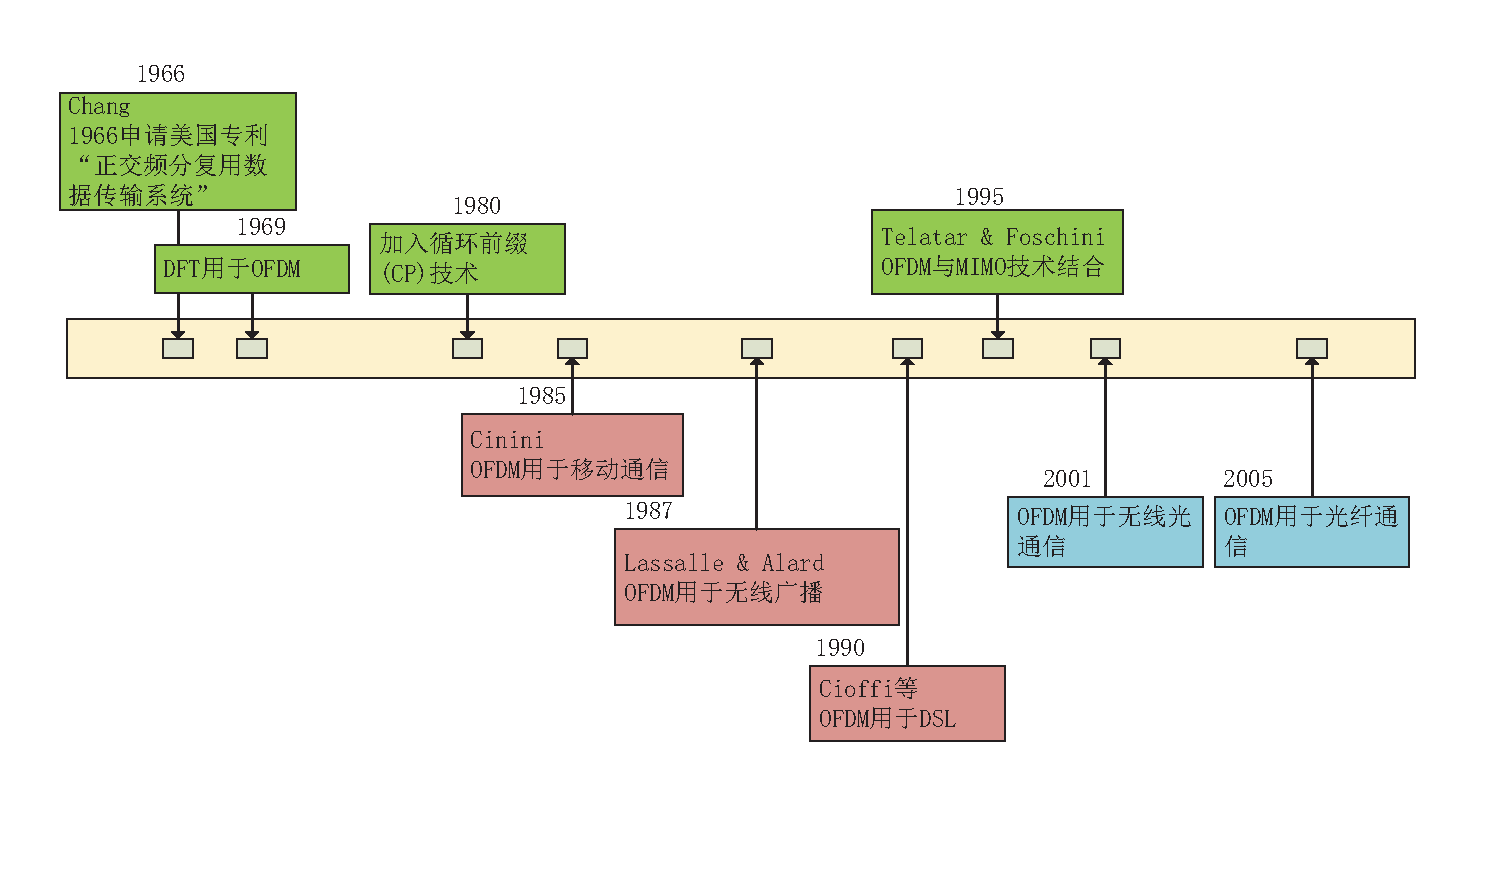
\includegraphics[width=0.8\textwidth]{figures/Chapter-2/HistoryOfOFDM.eps}
    \caption{OFDM技术发展历程及其应用}
    \label{fig:HistoryOfOFDM}
\end{figure}
\subsection{可见光中的OFDM调制}
\section{自适应传输技术简介}
\section{本章小结}
